\documentclass[prl,superscriptaddress,showpacs,twocolumn]{revtex4-1}
\usepackage{graphicx}
\usepackage{gensymb}
\usepackage{subfloat}
\usepackage{float}
\graphicspath{figures/}
	

\begin{document}
\title{Summary of Accuracy-Gated vs. Non-Gated Findings}
\author{Aaron Pache}

\maketitle

\noindent
\section{Energy vs. Accuracy/Error}
\begin{figure}[H]
    \centering
    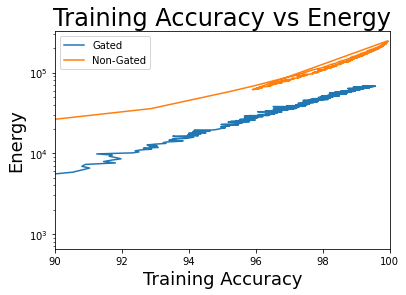
\includegraphics[width=\linewidth]{figures/training_accuracy_vs_energy.png}
    \caption{In training, the gated version provides reasonable energy saving over the non-gated version. The non-gated version, makes a sudden jump in accuracy from 99\% to 96\% and then climbs back up to 99\% accuracy.}
    \label{fig:train_acc_vs_energy}
\end{figure}

\begin{figure}[H]
    \centering
    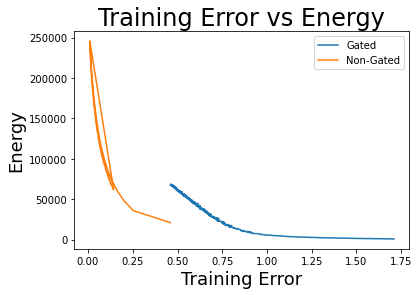
\includegraphics[width=\linewidth]{figures/training_error_vs_energy.png}
    \caption{As the training error gets smaller, energy rises exponentially.  I'm not sure if this would be the case for the gated version, since it never reaches a small enough error. Here, the accuracy jump from 99\% to 96\% in the non-gated version is visible through its training error. Later plots demonstrate this jump more clearly.}
    \label{fig:train_err_vs_energy}
\end{figure}

\begin{figure}[H]
    \centering
    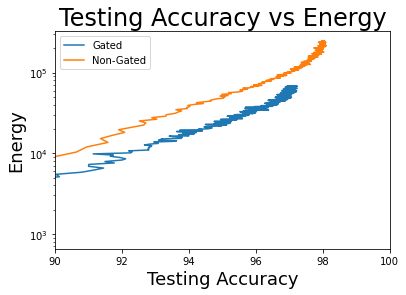
\includegraphics[width=\linewidth]{figures/testing_accuracy_vs_energy.png}
    \caption{At high accuracies, energy increases exponentially. The gated version begins to rise in energy at around 97\% but the non-gated version rises at around 98\%. Even still, the gated version sees energy-saving benefits.}
    \label{fig:test_acc_vs_energy}
\end{figure}

\begin{figure}[H]
    \centering
    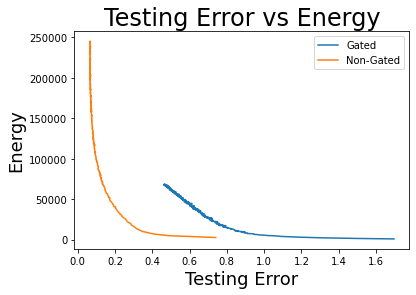
\includegraphics[width=\linewidth]{figures/testing_error_vs_energy.png}
    \caption{A similar, if not neater graph to its training counterpart (Figure \ref{fig:train_err_vs_energy}). At small errors the energy increases exponentially and slightly more dramatically compared to the training version. Again, it's difficult to say whether this is applicable to the gated version since it never reaches a low enough accuracy.}
    \label{fig:test_err_vs_energy}
\end{figure}

\section{Minimum Energy vs. Accuracy/Error}

\begin{figure}[H]
    \centering
    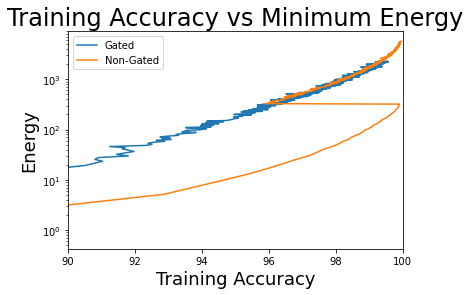
\includegraphics[width=\linewidth]{figures/training_accuracy_vs_minimum_energy.png}
    \caption{At minimum energy, the non-gated version consumes less energy. This probably suggests that while it \textit{could} find higher accuracies at lower energies, it doesn't and is therefore more inefficient, atleast in the training case. After this however, it traces the minimum energy of the gated version. I'm not sure if that means that they're taking the same path since the errors are so different...}
    \label{fig:train_acc_vs_min_energy}
\end{figure}

\begin{figure}[H]
    \centering
    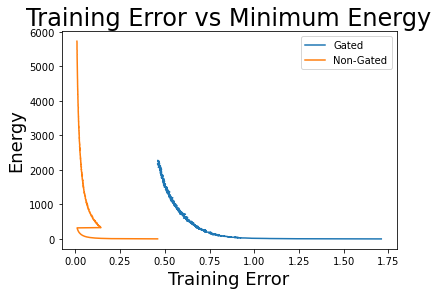
\includegraphics[width=\linewidth]{figures/training_error_vs_minimum_energy.png}
    \caption{Unlike the total energy, seen in Figure \ref{fig:train_err_vs_energy}, the minimum energy of the gated version increases exponentially at 0.5 error. While the non-gated version increases at 0.05. My guess is that high accuracies, require high energies but low errors require even higher energies. We infer the accuracy landscape from the error landscape but the error landscape is much more noisy at low errors.}
    \label{fig:train_err_vs_min_energy}
\end{figure}

\begin{figure}[H]
    \centering
    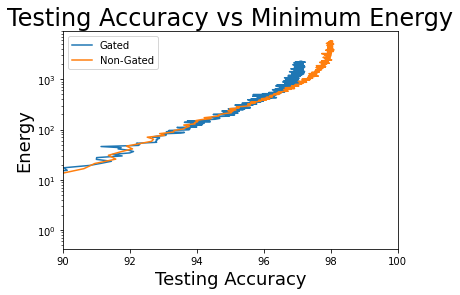
\includegraphics[width=\linewidth]{figures/testing_accuracy_vs_minimum_energy.png}
    \caption{Under the testing accuracy, both the gated and non-gated appear to walk a similar path until around 96\% accuracy. Here, the gated version is able to reach higher accuracies before exponentially increasing in energy. In comparison with the training version (Figure\ref{fig:train_acc_vs_min_energy}), it's clear that the non-gated version quickly overfits to the training data before finding a more globally applicable minima.}
    \label{fig:test_acc_vs_min_energy}
\end{figure}

\begin{figure}[H]
    \centering
    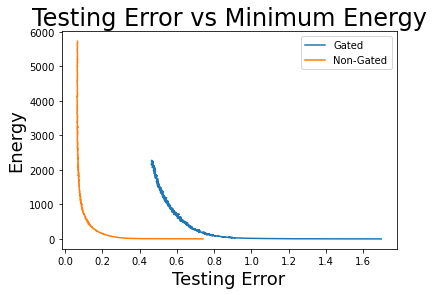
\includegraphics[width=\linewidth]{figures/testing_error_vs_minimum_energy.png}
    \caption{Again, like training error, the test error energy also increases exponentially for both the gated and non-gated version.}
    \label{fig:test_err_vs_min_energy}
\end{figure}

\section{Training Errors \& Accuracies vs. Testing Errors \& Accuracies}

\begin{figure}[H]
    \centering
    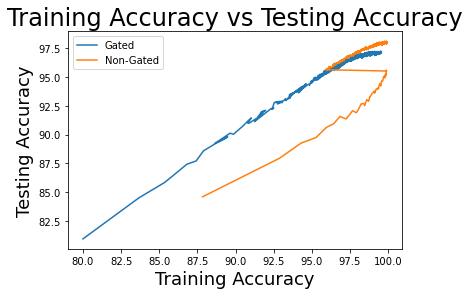
\includegraphics[width=\linewidth]{figures/training_accuracy_vs_testing_accuracy.png}
    \caption{The gated version follows a more linear path between testing and training accuracies but begins to overfit the training set at 97\% accuracy. The non-gated version is overfit from the start before finding a better gradient to traverse where it achieves a better testing accuracy than the gated version.}
    \label{fig:train_test_acc}
\end{figure}

\begin{figure}[H]
    \centering
    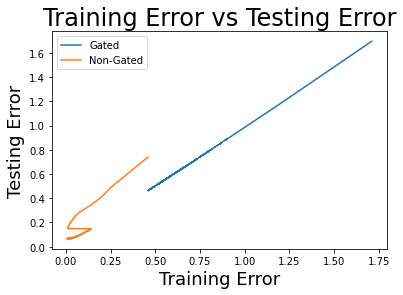
\includegraphics[width=\linewidth]{figures/training_error_vs_testing_error.png}
    \caption{The gated version does not overfit its training error and is surprisingly linear. The non-gated version overfits the training set error at around 0.1 error. }
    \label{fig:train_test_err}
\end{figure}

\section{An Intermission: My Thoughts}
As I allude to in Figure \ref{fig:train_err_vs_min_energy}, we're interested in the global accuracy landscape and we infer the training accuracy landscape from the training error landscape. I think that at high errors, the training/testing error landscapes are similar and smooth. As the training error decreases, past 0.3, the error landscape is much more noisy and therefore the training and testing errors begin to deviate. The gated version offers a regularisation effect to mitigate falling into this noisy mess by only correcting when necessary (i.e. incorrect samples), this traverses the error landscape much more slowly. \\
\indent
However, the error landscape is used to infer the accuracy landscape. Backpropagation provides a neat method of getting high accuracies following the assumption that 0 error = 100\% accuracy. However, it should be clear that the accuracy landscape is not equal to the error landscape. The error landscape contains the noise of every sample which is made explicit at lower errors. The accuracy landscape cuts through the error landscape at an angle and without noise (maybe low-pass filter?). Similar accuracies, but different errors between the gated and non-gated version exist because they lie on the same accuracy surface which cuts through the error surface, Figure \ref{fig:explanation} attempts to explain this with 1000 words. Unnecessary energy is expended tracking the error landscape of every sample and the least amount of energy likely traces the smoothest error gradient that cuts through each accuracy plane the fastest. Here, I'm imagining that each accuracy plane is like a slice at 90.0\%, 90.1\%, etc. (i.e. minimise error/maximise accuracy, this way little changes are made to the weights for the most amount of accuracy).\\

\begin{figure}[H]
    \centering
    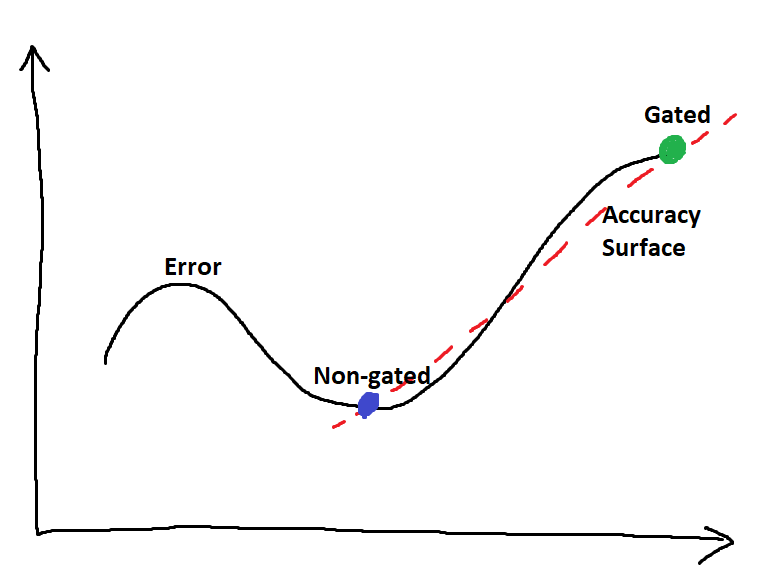
\includegraphics[width=\linewidth]{figures/explanation.png}
    \caption{The error landscape of a given sample. The blue dot represents the non-gated version's position on the error landscape and the green dot represents the gated version's position. The dotted red line represents points where the sample is correctly identified. (I feel like it's at the wrong angle but hopefully the point is conveyed). Energy has been expended bringing the blue ball down the hill, only for this minima to be destroyed on the next sample.}
    \label{fig:explanation}
\end{figure}

\indent
The analogy I internally use is that we each have our own unique handwriting because we lie on the 100\% accuracy plane not the 0 error plane. I think a teacher would expend much more energy explaining every detail on how a student should perfectly copy the teacher's `a'.


\section{Samples vs. Accuracy/Error \& Training/Testing}
\begin{figure}[H]
    \centering
    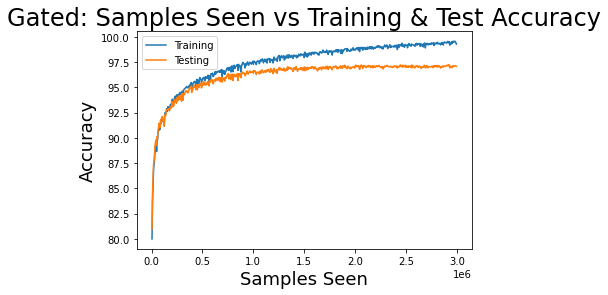
\includegraphics[width=\linewidth]{figures/gated_samples_vs_train_test_accuracy.png}
    \caption{The gated version begins to overfit the training set accuracy at around 96\% accuracy and is able to achieve this accuracy after 750,000 training samples or 12.5 epochs.}
    \label{fig:gated_acc}
\end{figure}

\begin{figure}[H]
    \centering
    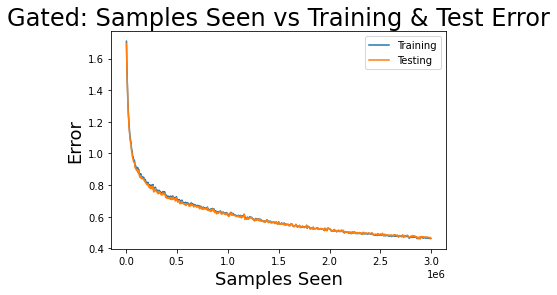
\includegraphics[width=\linewidth]{figures/gated_samples_vs_train_test_error.png}
    \caption{The gated version does not overfit to the training error landscape, both remain equal for all samples seen and trained against.}
    \label{fig:gated_err}
\end{figure}

\vspace{5cm}
\newpage

\begin{figure}[H]
    \centering
    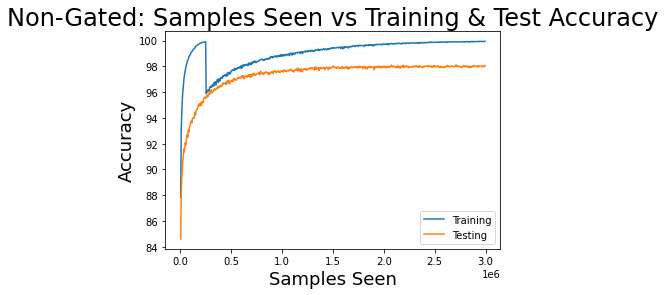
\includegraphics[width=\linewidth]{figures/non_gated_samples_vs_train_test_accuracy.png}
    \caption{The non-gated version overfits rapidly, corrects and begins to overfit again. It achieves 96\% accuracy at around 250,000 samples or 4.1 epochs.}
    \label{fig:non_gated_acc}
\end{figure}

\begin{figure}[H]
    \centering
    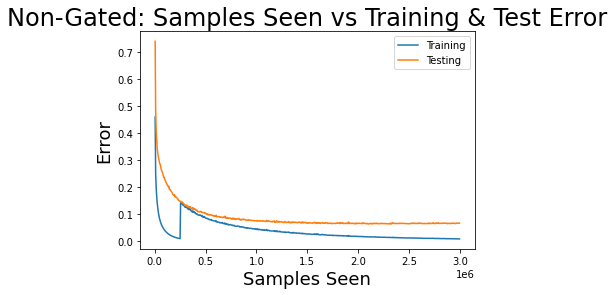
\includegraphics[width=\linewidth]{figures/non_gated_samples_vs_train_test_error.png}
    \caption{The non-gated version also overfits the training set's error landscape, unlike the gated version (Figure \ref{fig:gated_err}).}
    \label{fig:non_gated_err}
\end{figure}

\clearpage

\begin{figure}[H]
    \centering
    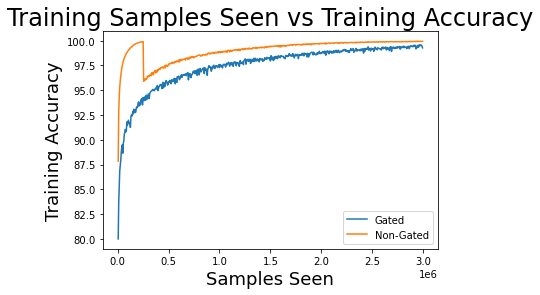
\includegraphics[width=\linewidth]{figures/samples_vs_training_accuracy.png}
    \caption{The non-gated version is able to reach a higher accuracy with less samples seen, 96\% accuracy is achieved with 250,000 samples while the gated version takes 750,000 samples.}
    \label{fig:train_acc}
\end{figure}

\begin{figure}[H]
    \centering
    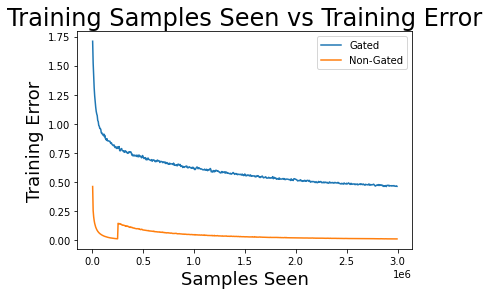
\includegraphics[width=\linewidth]{figures/samples_vs_training_error.png}
    \caption{Again, the non-gated version is capable of reaching a low error with little samples. The gated version prevents the error from getting too low and doesn't saturate as quickly.}
    \label{fig:train_err}
\end{figure}

\vspace{5cm}
\newpage

\begin{figure}[H]
    \centering
    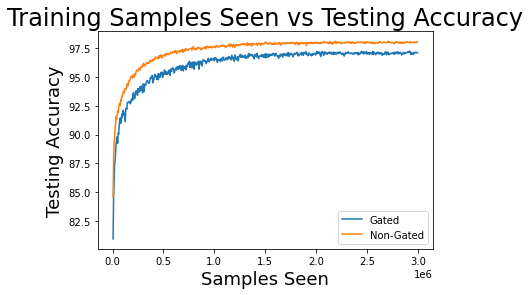
\includegraphics[width=\linewidth]{figures/samples_vs_testing_accuracy.png}
    \caption{The non-gated version is able to achieve a higher testing accuracy than the gated version and has a faster rise time. Even though, from Figure \ref{fig:train_acc}, the gated version increases in training accuracy, this does not translate to testing accuracy suggesting it has overfit to the training accuracy plane.}
    \label{fig:test_acc}
\end{figure}

\begin{figure}[H]
    \centering
    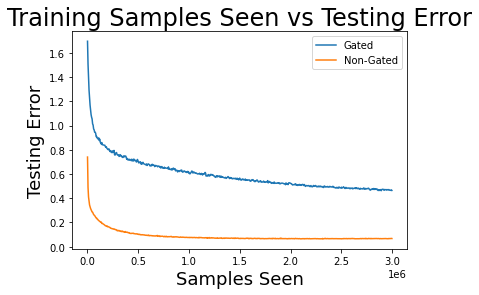
\includegraphics[width=\linewidth]{figures/samples_vs_testing_error.png}
    \caption{A similar plot to Figure \ref{fig:train_err}, the training error version and a similar description would be given here too.}
    \label{fig:test_err}
\end{figure}

I think these plots further corroborate that the training/testing error surfaces are smooth and similar at errors greater than 0.4. From Figures \ref{fig:gated_err}, \ref{fig:non_gated_err}, \ref{fig:train_err} and \ref{fig:test_err}, the errors are similar above 0.4 and overfitting occurs under 0.4. (although, the non-gated version quickly drops below this, so I'm unsure how applicable this extrapolation is). \\
\indent
I think that they also show the global accuracy landscape and global error landscape are similar above 0.75, which is when the gated version begin to deviate in Figure \ref{fig:gated_acc}. I'm not sure how similar they are beyond these points, but I think the accuracy landscape is smoother than the error landscape beyond these points. \\
\indent
I think the challenge is now: how do we navigate the accuracy surface? 

\end{document}

